\section{Introduction}
\label{sec:intro}

Lithium-ion batteries power electric vehicles, grid-scale energy
storage, spacecraft, and portable electronics, and the market they
serve is projected to grow several-fold over the coming decade
\cite{ref_yang_review,ref_sbarra_dt}---making battery health
management a first-order economic concern rather than a technical
nicety. Each application stresses battery management differently:
electric-vehicle packs must track health under rapidly varying
current, temperature, and state of charge, where capacity fade
shortens range and raises thermal-safety risk; grid-scale storage
integrates hundreds of thousands of cells into hierarchical
cell--pack--cluster--container systems, where single-cell aging
accumulates into fleet-level inconsistency that dominates life-cycle
operating cost \cite{ref_qu_bess}; spacecraft batteries must operate
for years without on-site repair under radiation, vacuum, and
extreme temperatures, where power-subsystem anomalies are a leading
cause of mission loss \cite{ref_sbarra_dt}; and portable electronics
make battery health the most ubiquitous---and least
supervised---monitoring problem of all.

Battery management systems (BMS) distill battery health into three
state quantities: \emph{state of charge} (SOC), the fraction of
remaining usable charge---the ``fuel gauge''; \emph{state of health}
(SOH), the current full capacity relative to rated capacity---the
``health report,'' whose convention-specified end-of-life threshold
(typically 70--80\% of rated capacity) defines retirement; and
\emph{remaining useful life} (RUL), the number of cycles until that
threshold is crossed---the ``countdown.'' The three form a
progression: SOC describes how much energy remains now, SOH how far
aging has progressed, and RUL how long the asset will keep serving;
of the three, RUL is the forward-looking quantity that maintenance
and replacement decisions actually consume
\cite{ref_yang_review,ref_sbarra_dt}.

That progression rests on a fundamental contradiction: the chemistry
prized for its high energy density and long cycle life ages
inevitably under use. Two microscopic mechanisms dominate the
aging---\emph{loss of lithium inventory}, as the growing
solid-electrolyte interface consumes cyclable lithium, and
\emph{loss of active material}, as electrode particles crack and
detach---and both manifest macroscopically as capacity fade and
rising internal resistance \cite{ref_yang_review}. The resulting
degradation is inherently nonlinear and heterogeneous: a long-term
monotonic fade is intertwined with capacity regeneration events,
stage-wise transitions, and measurement noise, making RUL prediction
a challenging prognostics problem \cite{ref_rulmamba,ref_omnitie}.
The battery's internal state is moreover a black box: health
indicators must be inferred from external measurements rather than
observed directly, which is why health prediction is inherently
uncertain---and why an estimator that consumes only
field-measurable quantities has direct operational value.

For operators, RUL is far more than an academic metric. It converts
maintenance from reactive repair to planned intervention; it informs
retirement and second-life decisions that extend a battery's
economic life; it bounds safety margins, since capacity fade and
resistance rise are recognized precursors of thermal runaway; and it
caps life-cycle cost, the dominant expense of large storage fleets
\cite{ref_yang_review,ref_qu_bess}.

Existing RUL prediction methods fall into two broad families.
Model-based approaches---equivalent-circuit models, extended and
unscented Kalman filters, and particle filters---encode degradation
physics explicitly \cite{ref_ekf_yan,ref_upf_cong,ref_pf_echem,
ref_pf_rbf,ref_pf_lui} but require accurate parameter identification
and often lack the flexibility to capture regeneration dynamics.
Data-driven approaches learn degradation patterns directly from
cycling data. Within this family, recurrent networks (LSTM, GRU)
\cite{ref_lstm_transformer,ref_lstm_rul_zhang,ref_gru_ding} model
sequential capacity evolution but suffer from long-term dependency
limitations \cite{ref_rulmamba}; Transformer-based models
\cite{ref_vaswani} such as PatchFormer \cite{ref_patchformer}
and general time-series transformers \cite{ref_autoformer}
\cite{ref_fedformer} achieve strong accuracy but their quadratic
attention complexity and growing memory footprint hinder deployment
on resource-constrained embedded platforms. Most recently, state
space models (SSMs) such as Mamba \cite{ref_mamba} have been applied
to battery prognostics, with RUL-Mamba \cite{ref_rulmamba} reporting
state-of-the-art performance on NASA, Oxford, and TJU datasets---yet
the reported efficiency is measured on GPUs, and edge-deployment
feasibility is not addressed.

Despite these advances, four limitations remain. First, quadratic
self-attention makes Transformer-based models difficult to deploy on
microcontrollers (MCUs) used in BMS: the attention score matrix grows
with sequence length, requiring dynamic memory allocation that is
undesirable in safety-critical firmware. Second, degradation
information lives at multiple time scales---fast regeneration
events, intermediate stage transitions, and the slow monotonic
fade---and models that treat the capacity sequence as a single scale
either over-smooth the recoveries or lose the global trend
\cite{ref_omnitie}. Third, purely data-driven models are evaluated on clean
laboratory data and falter exactly where field operation deviates
from the lab: the end-of-life acceleration tail---where maintenance
decisions concentrate---is the regime with the least training data,
so learned predictors flatten or drift there, and corrupted or noisy
sensor streams sharply degrade their predictions. Fourth, point
estimates of SOH and RUL do not convey uncertainty, which limits
their use in risk-aware BMS decisions.

Beneath these technical gaps lies a decision-layer gap: even an
accurate SOH/RUL estimate is an intermediate product, and translating
it into maintenance actions today still relies on expert judgment.
Field evidence from large-scale storage systems shows that
explainable, decision-oriented operation and maintenance frameworks
cut response time and operational cost by over 80\% compared with
conventional expert-driven practice \cite{ref_qu_bess}. The extreme
operating regime is space: the vast majority of new satellites run
on lithium-ion batteries, in-orbit repair is impossible, and
power-subsystem anomalies are a leading cause of satellite faults
\cite{ref_sbarra_dt}---an environment where on-device, decision-grade
prognostics is a requirement rather than a convenience.

This paper proposes \emph{DeltaCycle}, a multi-scale linear-attention
network for battery prognostics designed from the outset for embedded
deployment. Our contributions are:

\begin{enumerate}
\item \textbf{Linear-attention backbone with verified edge
deployment.} We adopt Gated DeltaNet-2 (GDN-2), a recurrent linear
attention layer with a fixed-size matrix state (8\,KB per layer in
the deployed configuration), and ship a full C
implementation that matches the PyTorch forward within
floating-point rounding, with arithmetic and libm components
verified bit-identical across x86 and ARM emulation. \emph{Operationally, the
accuracy machinery is no longer tied to the cloud: the model runs
inside the BMS microcontroller itself---the prerequisite for
per-device monitoring at fleet scale and near-zero marginal cost.}

\item \textbf{Multi-scale branches with stage-query cross-scale
exchange.} Three patch branches (sizes 2/4/8) read degradation at
local, regional, and global scales; after every layer the coarse
branch's GDN state---the compressed degradation history---projects to
a single query that reads the fine and mid branch sequences.
Ablations show the exchange is essential. \emph{Operationally, the
coarse branch acts as an explicit degradation-stage indicator---the
piece of information maintenance scheduling actually consumes.}

\item \textbf{A physics-consistent degradation-rate head.} Why
physics at all? The third limitation above is the motivation:
learned predictors flatten or drift exactly where the data is
thinnest, and physics supplies an inductive bias that remains valid
outside the observed distribution---capacity decay is monotone, and
internal resistance can only accelerate it. The challenge is
injecting that bias without breaking the standard evaluation
protocol. A systematic injection-route study shows why conventional
physics injection fails under that protocol (the z-score target
space is structurally incompatible with monotone predictors), and
yields the mechanism that \emph{does} work: a rate head driven
by measured internal resistance, constrained so that resistance can
only accelerate decay, trained in absolute capacity space. The contribution is the
physics itself, and its value is demonstrated where physics should
matter: unseen-tail extrapolation fidelity doubles and the head wins
every corruption-robustness setting tested---evidence that the
mechanism is doing measurable work rather than acting as a
decorative constraint.

\item \textbf{Decision-grade uncertainty at one forward pass.} A
single pinball-trained model emits P2.5/P50/P97.5 intervals;
conformal calibration on a held-out cell lifts coverage to $93.3\%$
at nominal $95\%$, with two scalars and no ensemble. \emph{The
interval, not the point estimate, is what a replacement policy
consumes: the calibrated band bounds the missed-EOL rate that a
risk-averse scheduler actually cares about.}
\end{enumerate}

\begin{figure}[htbp]
\centering
% Row 1: six deployment contexts (photos)
\begin{subfigure}[b]{0.155\textwidth}
\centering
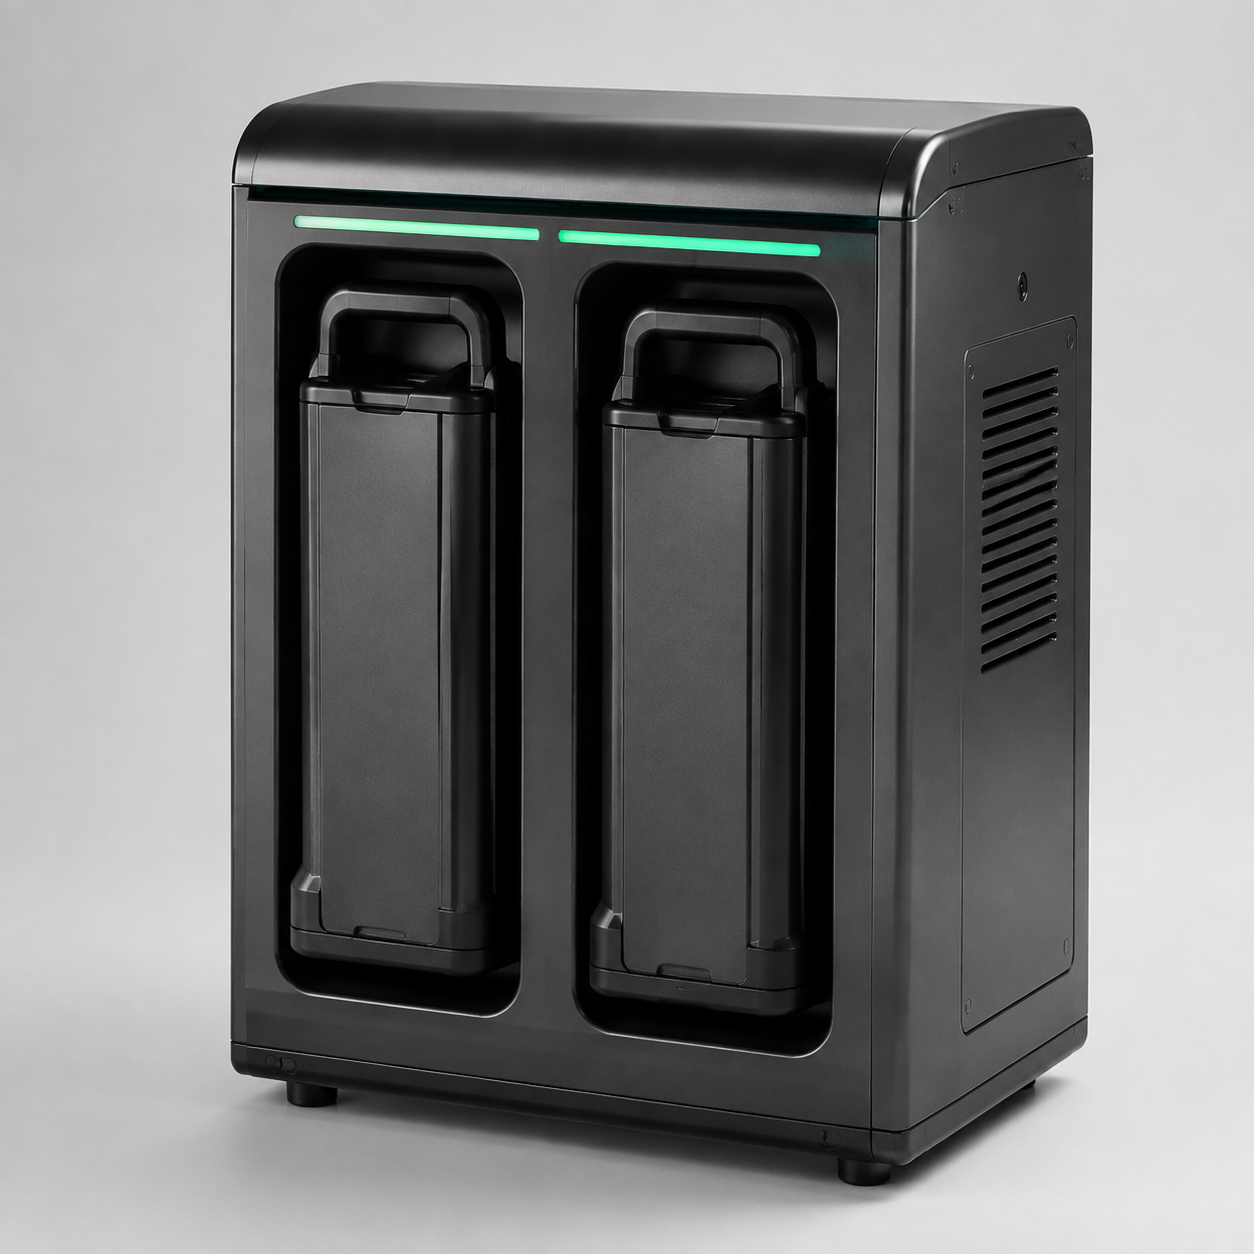
\includegraphics[width=\linewidth]{figures/ov_app1}
\caption{E-bike swap}\label{fig:ov_app1}
\end{subfigure}\hfill
\begin{subfigure}[b]{0.155\textwidth}
\centering
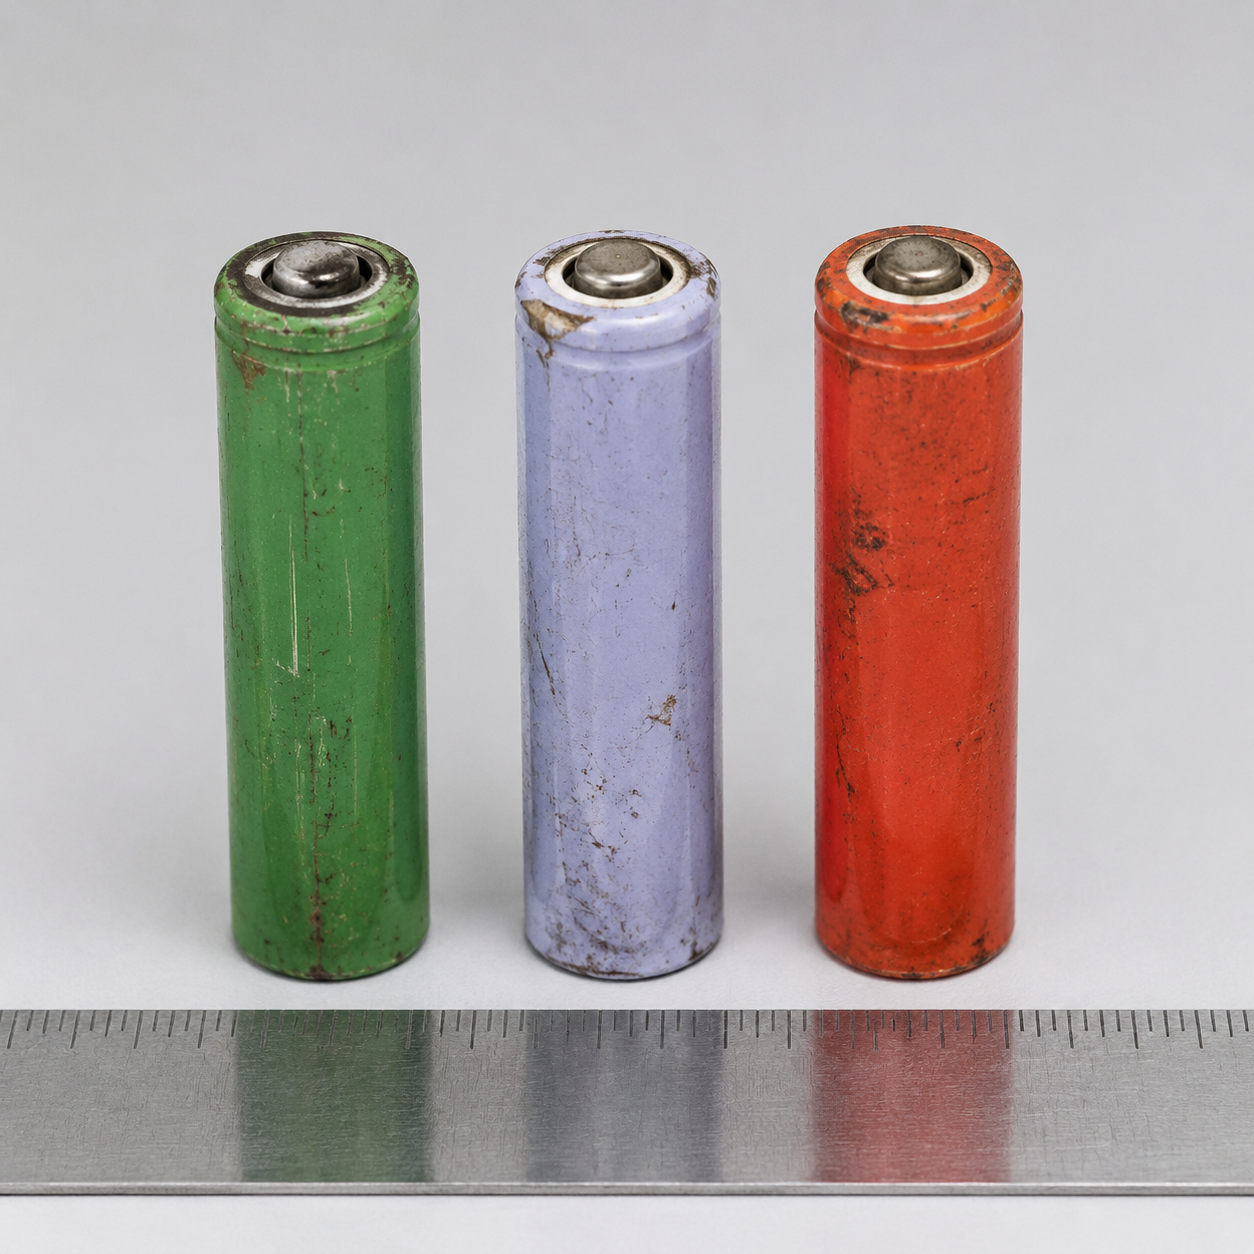
\includegraphics[width=\linewidth]{figures/ov_app2}
\caption{Second life}\label{fig:ov_app2}
\end{subfigure}\hfill
\begin{subfigure}[b]{0.155\textwidth}
\centering
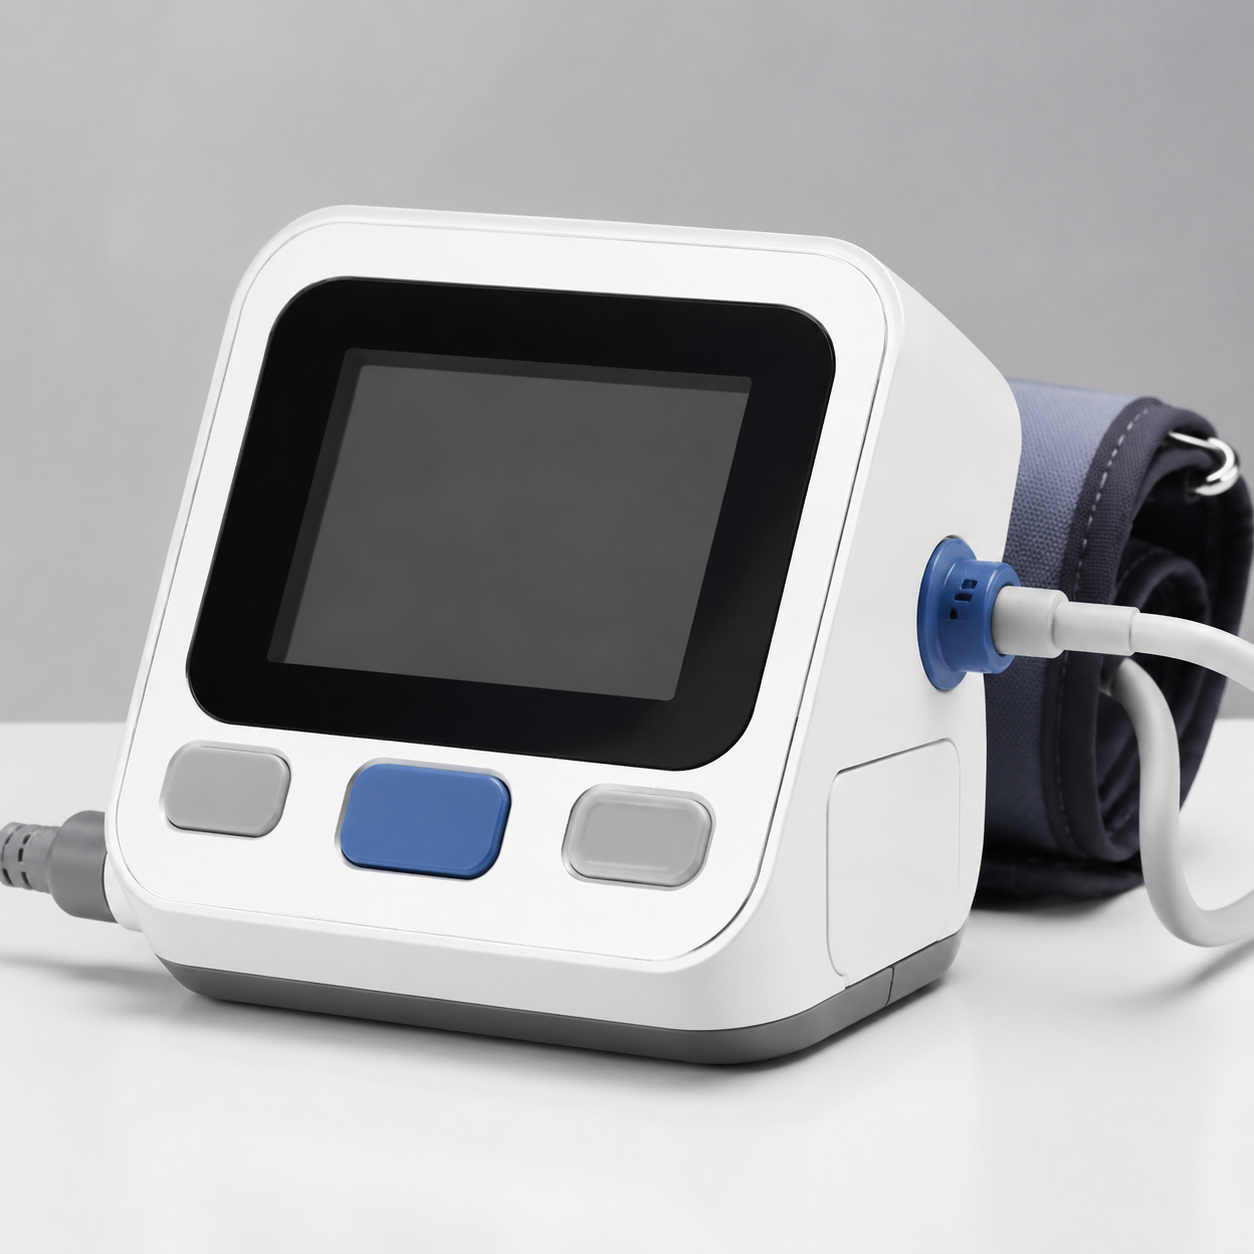
\includegraphics[width=\linewidth]{figures/ov_app3}
\caption{Portable medical}\label{fig:ov_app3}
\end{subfigure}\hfill
\begin{subfigure}[b]{0.155\textwidth}
\centering
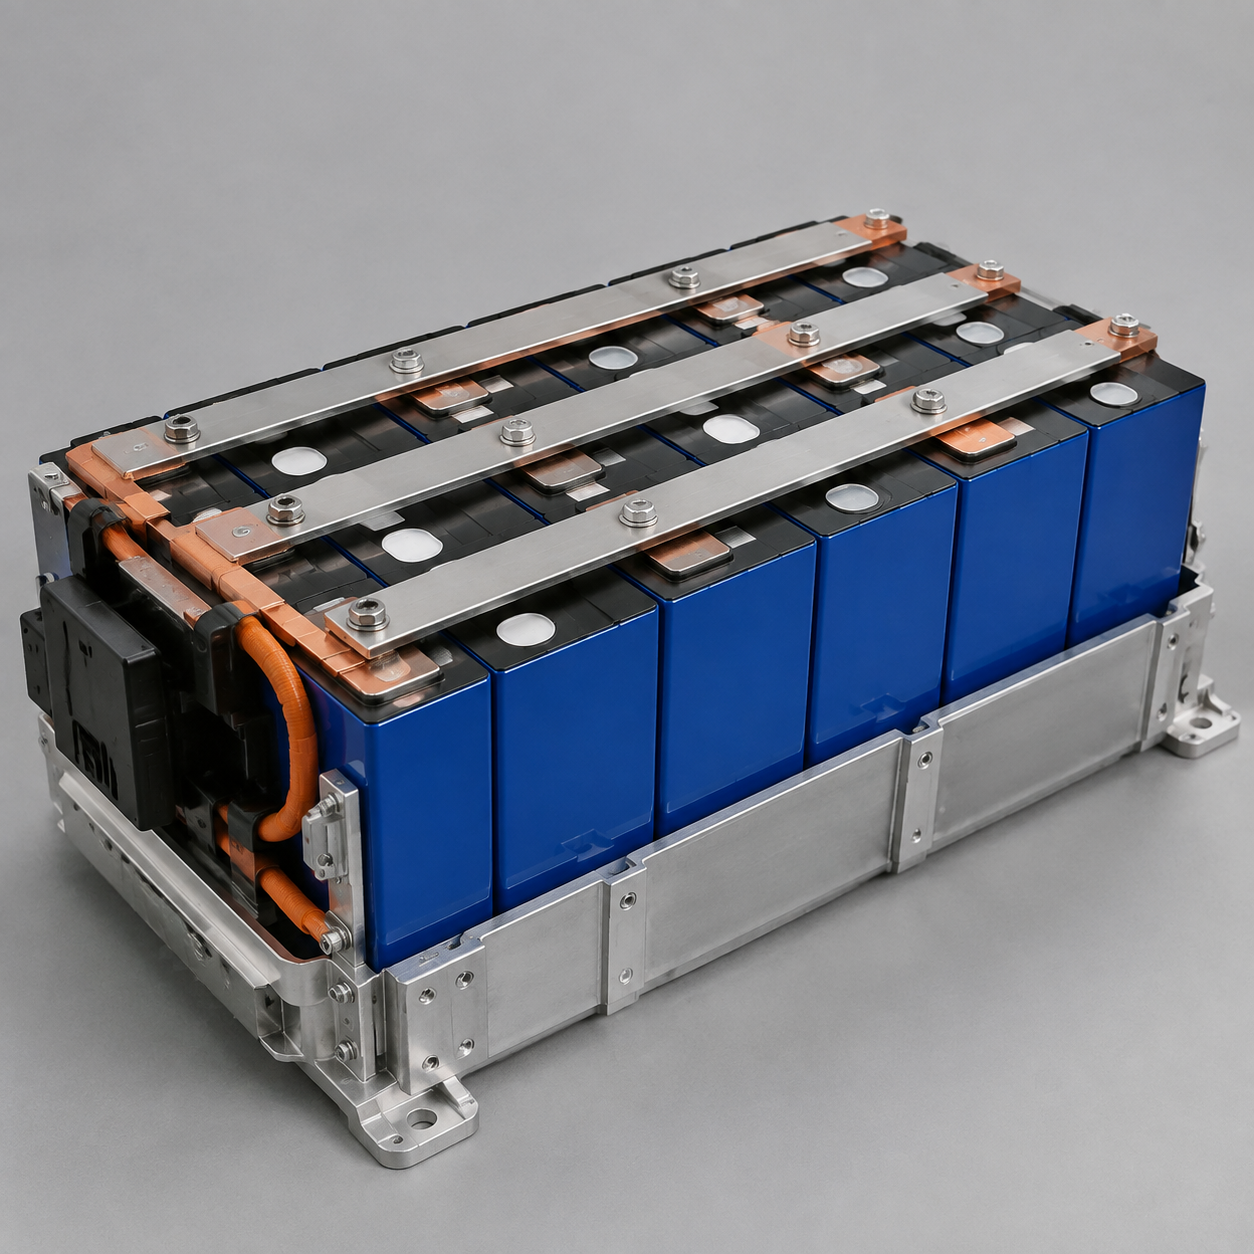
\includegraphics[width=\linewidth]{figures/ov_app4}
\caption{EV fleet}\label{fig:ov_app4}
\end{subfigure}\hfill
\begin{subfigure}[b]{0.155\textwidth}
\centering
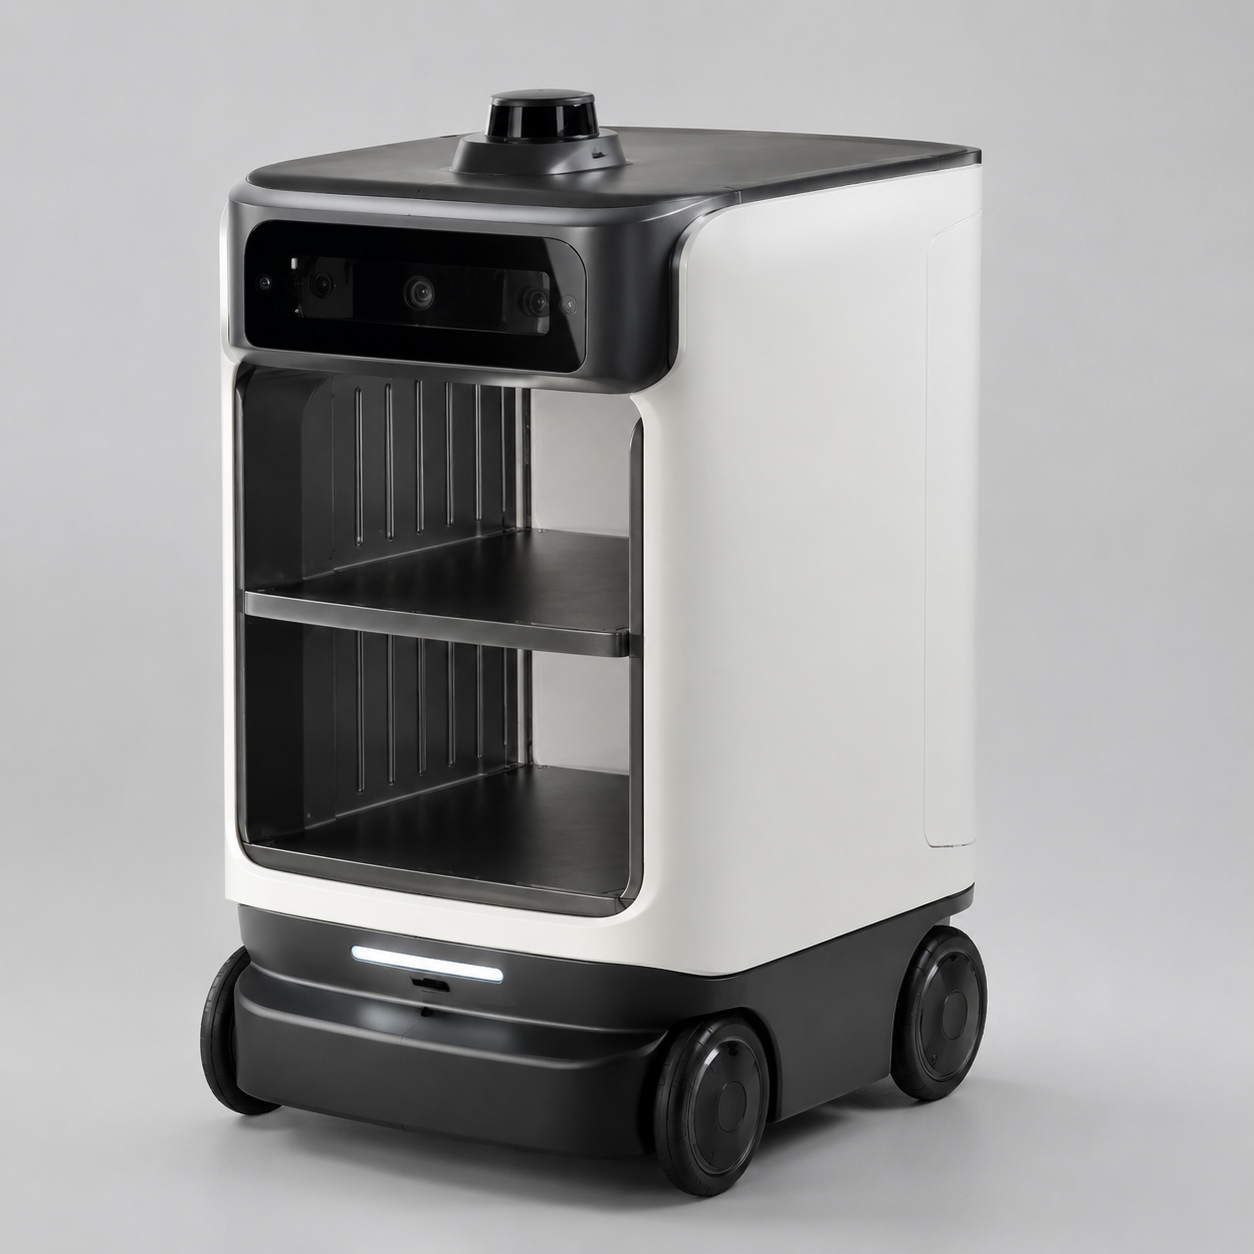
\includegraphics[width=\linewidth]{figures/ov_app5}
\caption{Robot fleet}\label{fig:ov_app5}
\end{subfigure}\hfill
\begin{subfigure}[b]{0.155\textwidth}
\centering

\includegraphics[width=\linewidth]{figures/ov_app6}
\caption{Power tools}\label{fig:ov_app6}
\end{subfigure}

\medskip
% Row 2: model pipeline (wider tiles)
\begin{subfigure}[b]{0.31\textwidth}
\centering
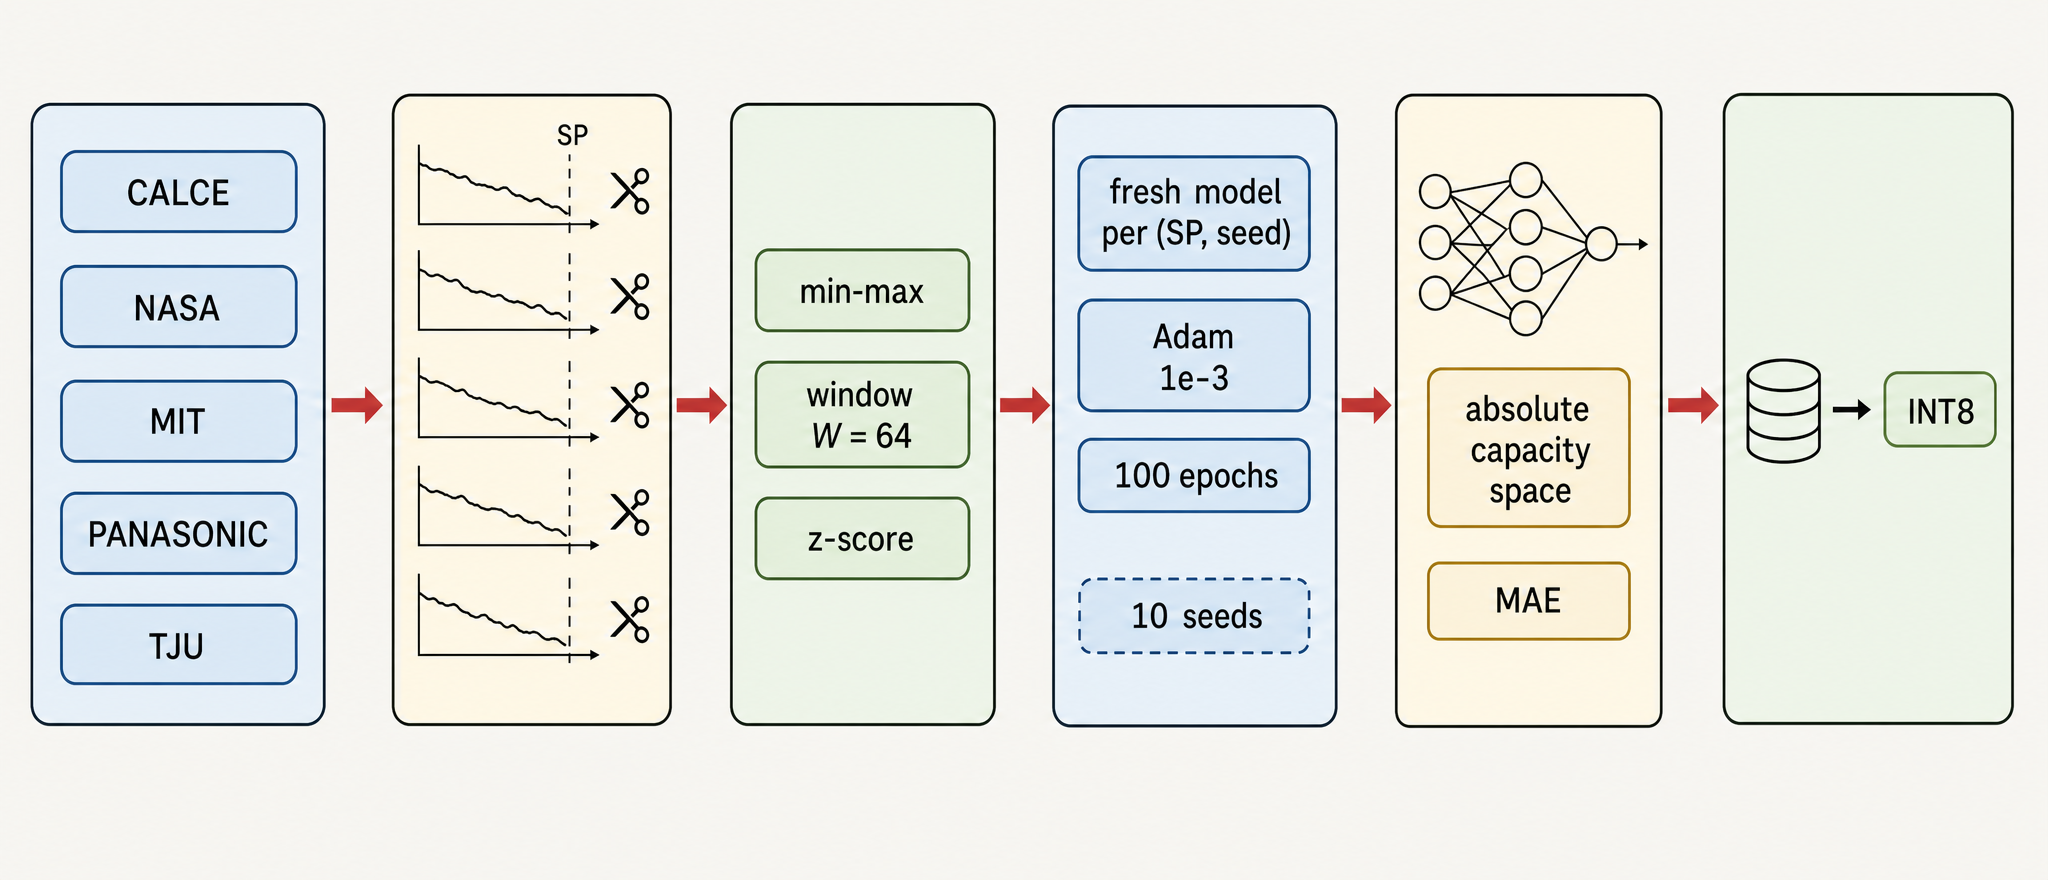
\includegraphics[width=\linewidth]{figures/ov_ms_train}
\caption{Training}\label{fig:ov_attr_train}
\end{subfigure}\hfill
\begin{subfigure}[b]{0.31\textwidth}
\centering
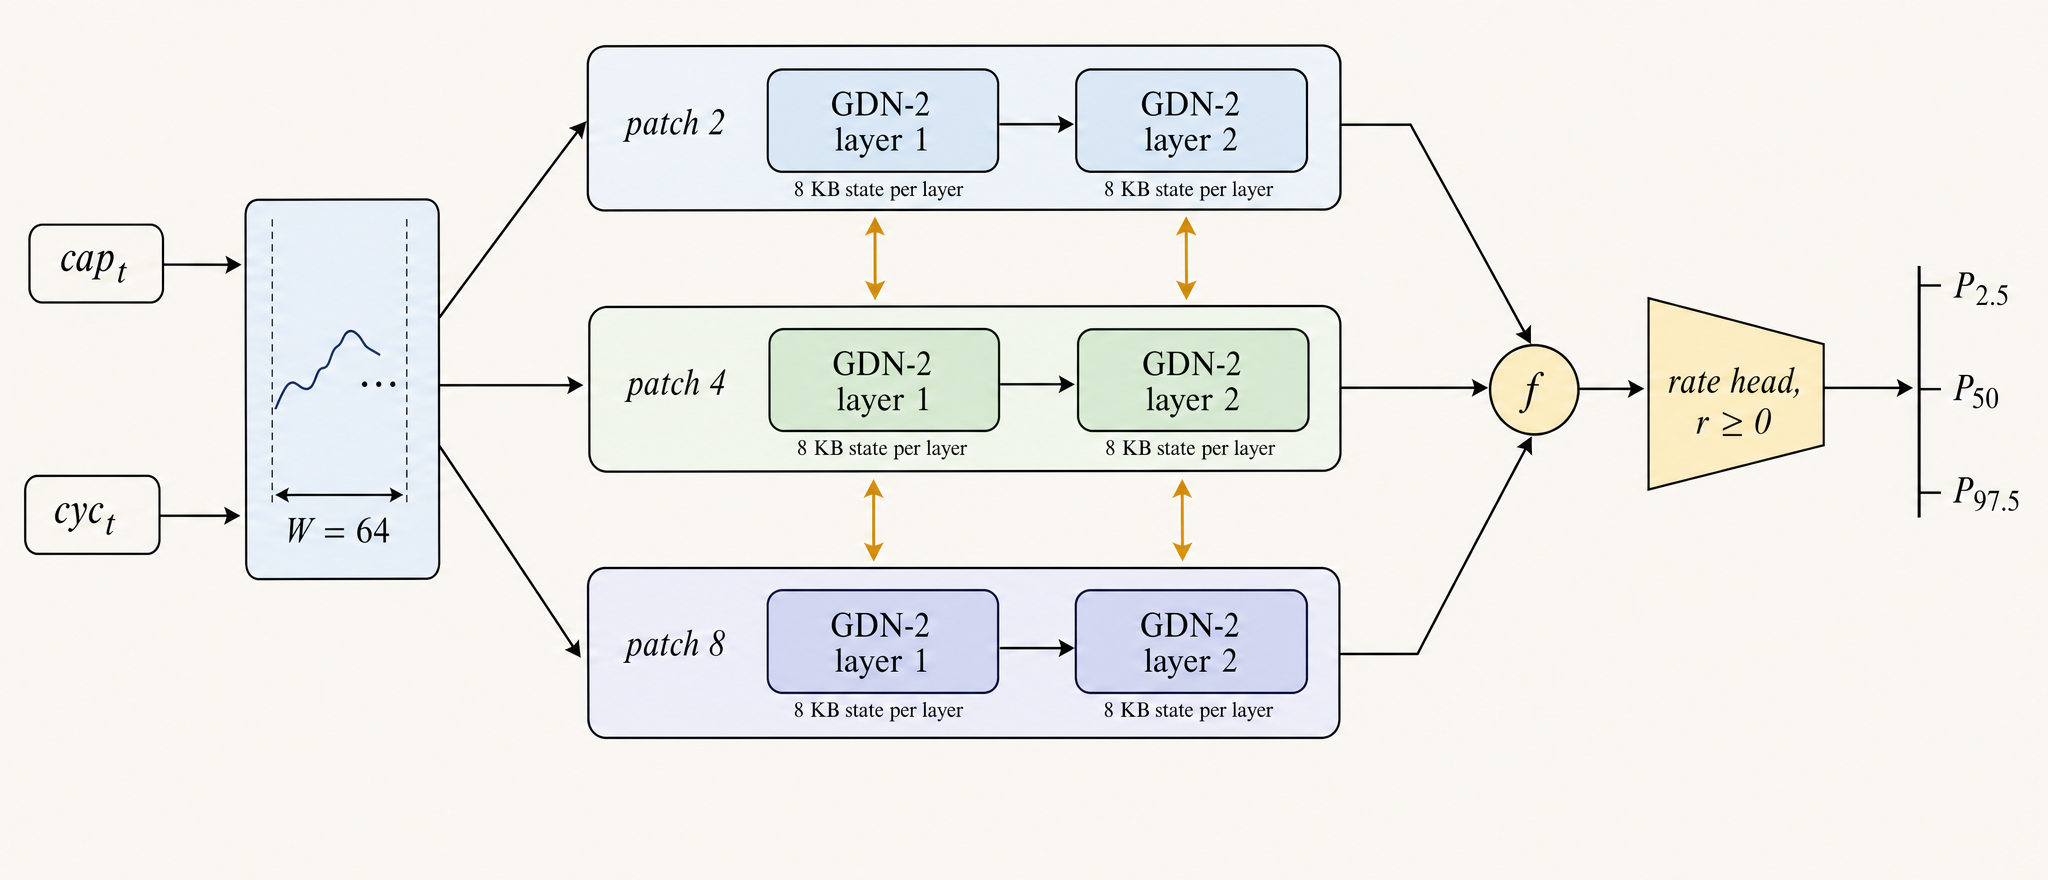
\includegraphics[width=\linewidth]{figures/ov_ms_model}
\caption{Model structure}\label{fig:ov_attr_model}
\end{subfigure}\hfill
\begin{subfigure}[b]{0.31\textwidth}
\centering
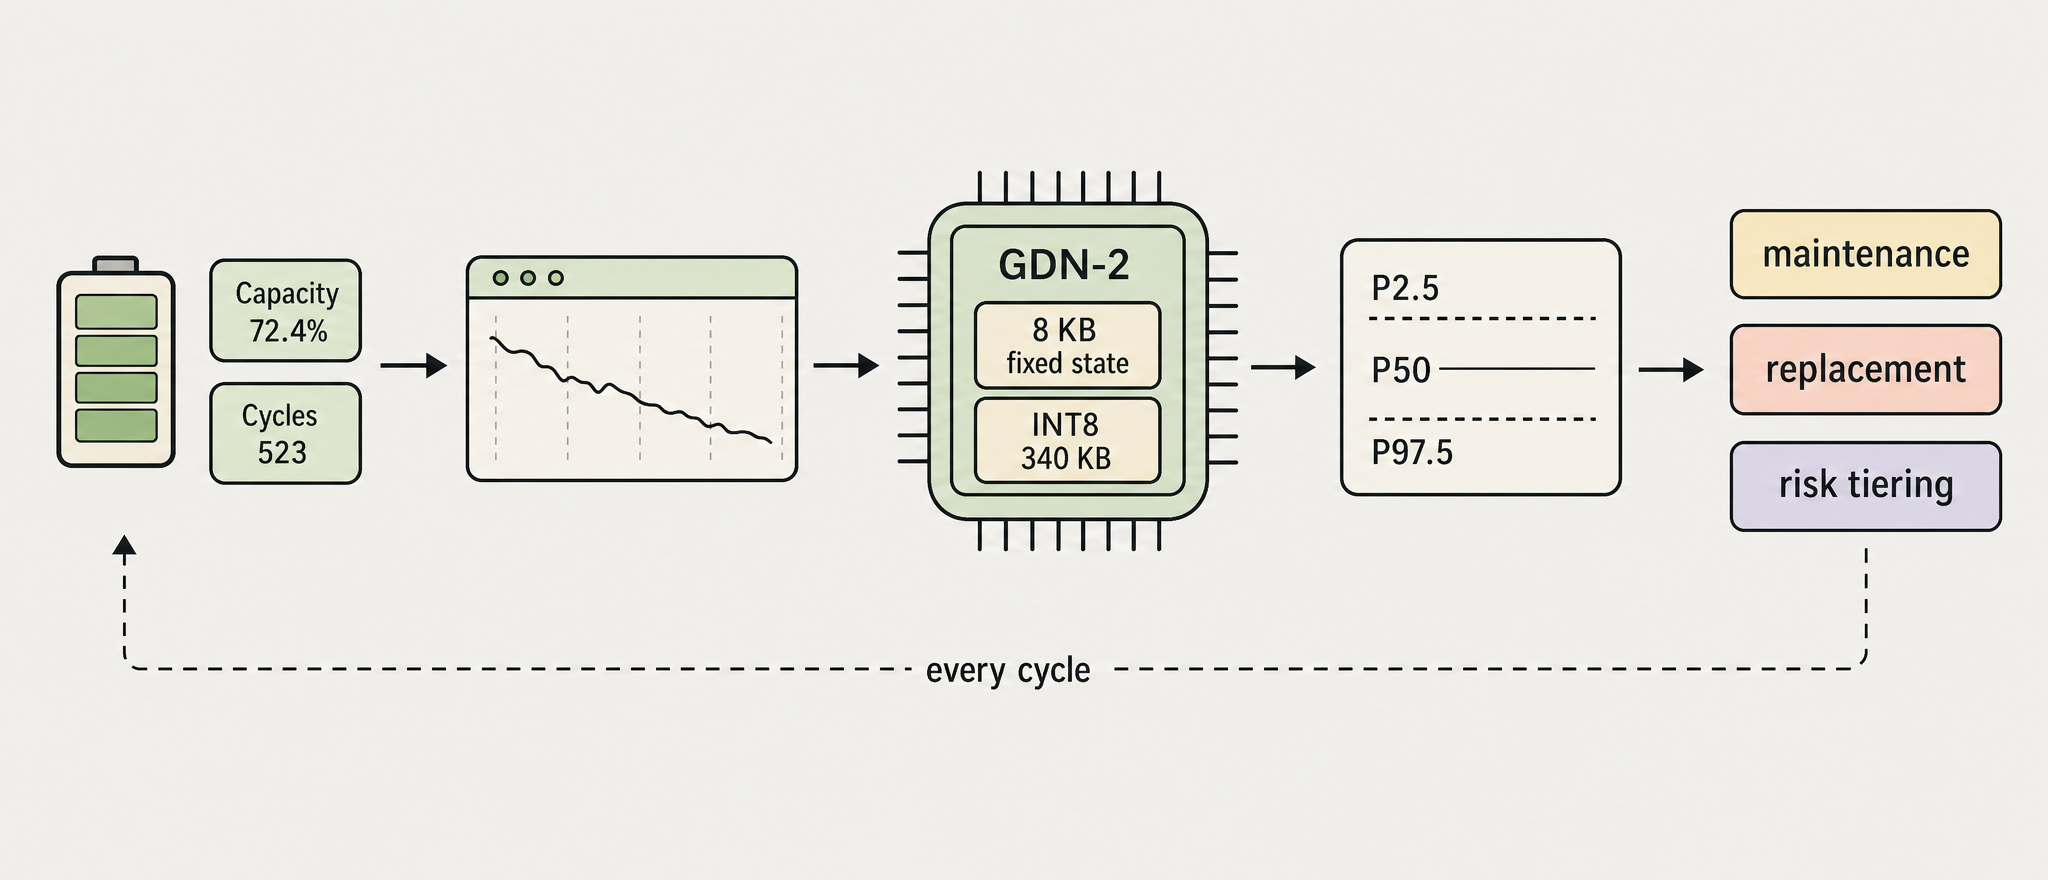
\includegraphics[width=\linewidth]{figures/ov_ms_infer}
\caption{Inference}\label{fig:ov_attr_infer}
\end{subfigure}

\medskip
% Row 3: four capabilities (A-D)
\begin{subfigure}[b]{0.235\textwidth}
\centering

\includegraphics[width=\linewidth]{figures/ov_p3a}
\caption{First-tier accuracy}\label{fig:ov_attr_acc}
\end{subfigure}\hfill
\begin{subfigure}[b]{0.235\textwidth}
\centering
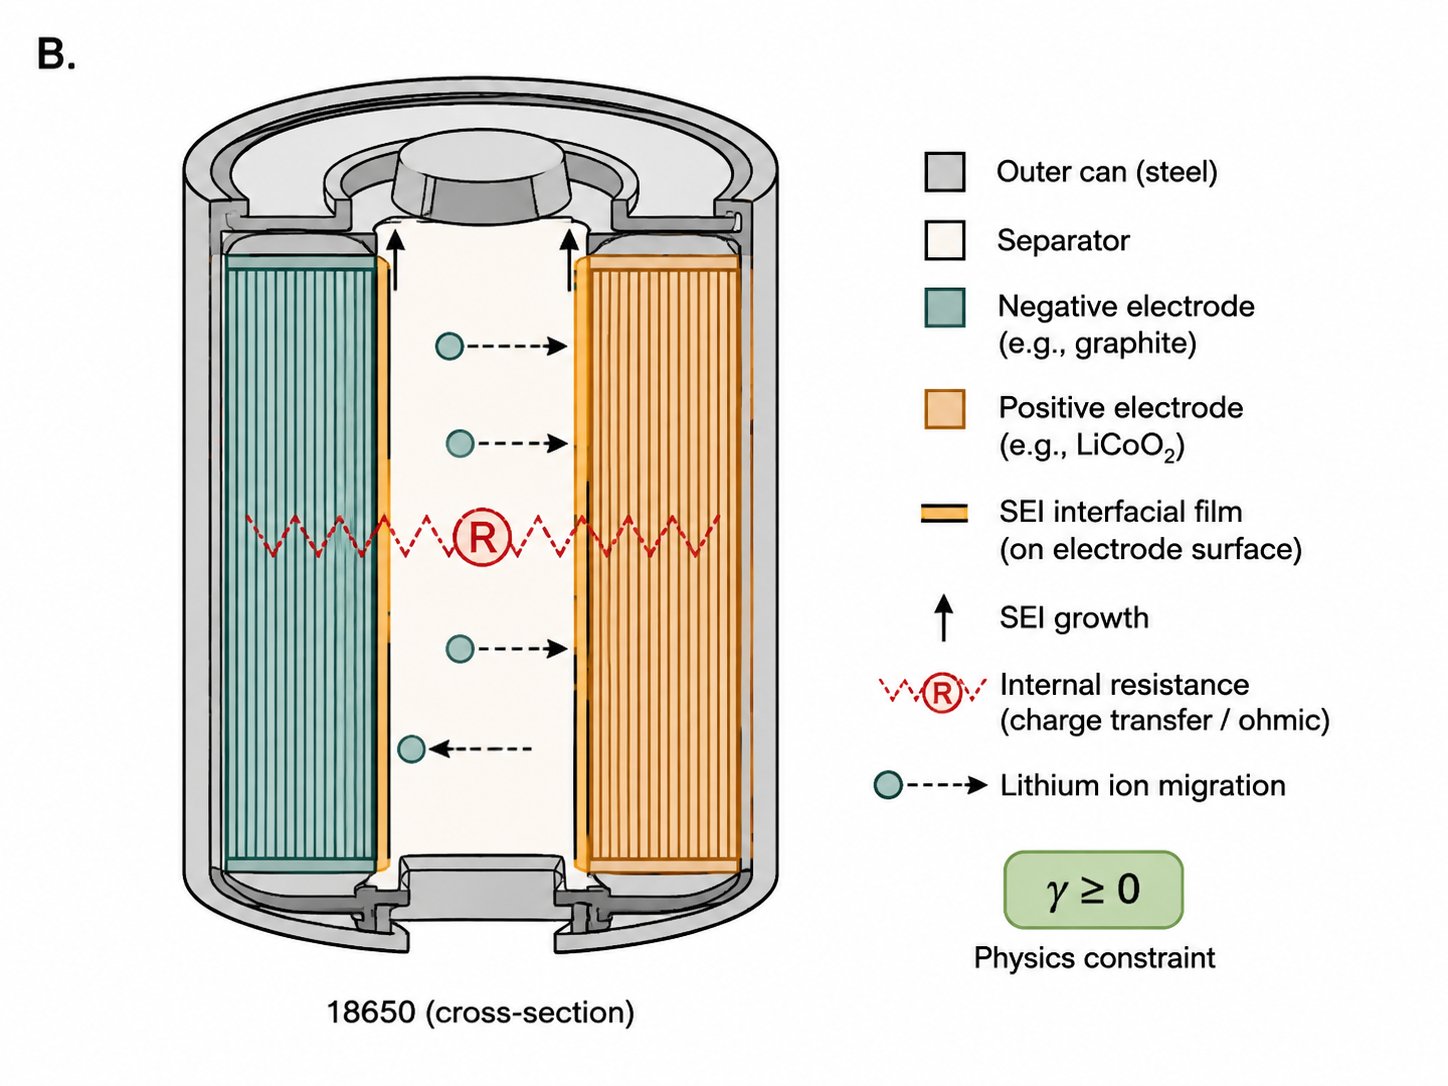
\includegraphics[width=\linewidth]{figures/ov_p3b}
\caption{Physics-consistent head}\label{fig:ov_attr_phys}
\end{subfigure}\hfill
\begin{subfigure}[b]{0.235\textwidth}
\centering
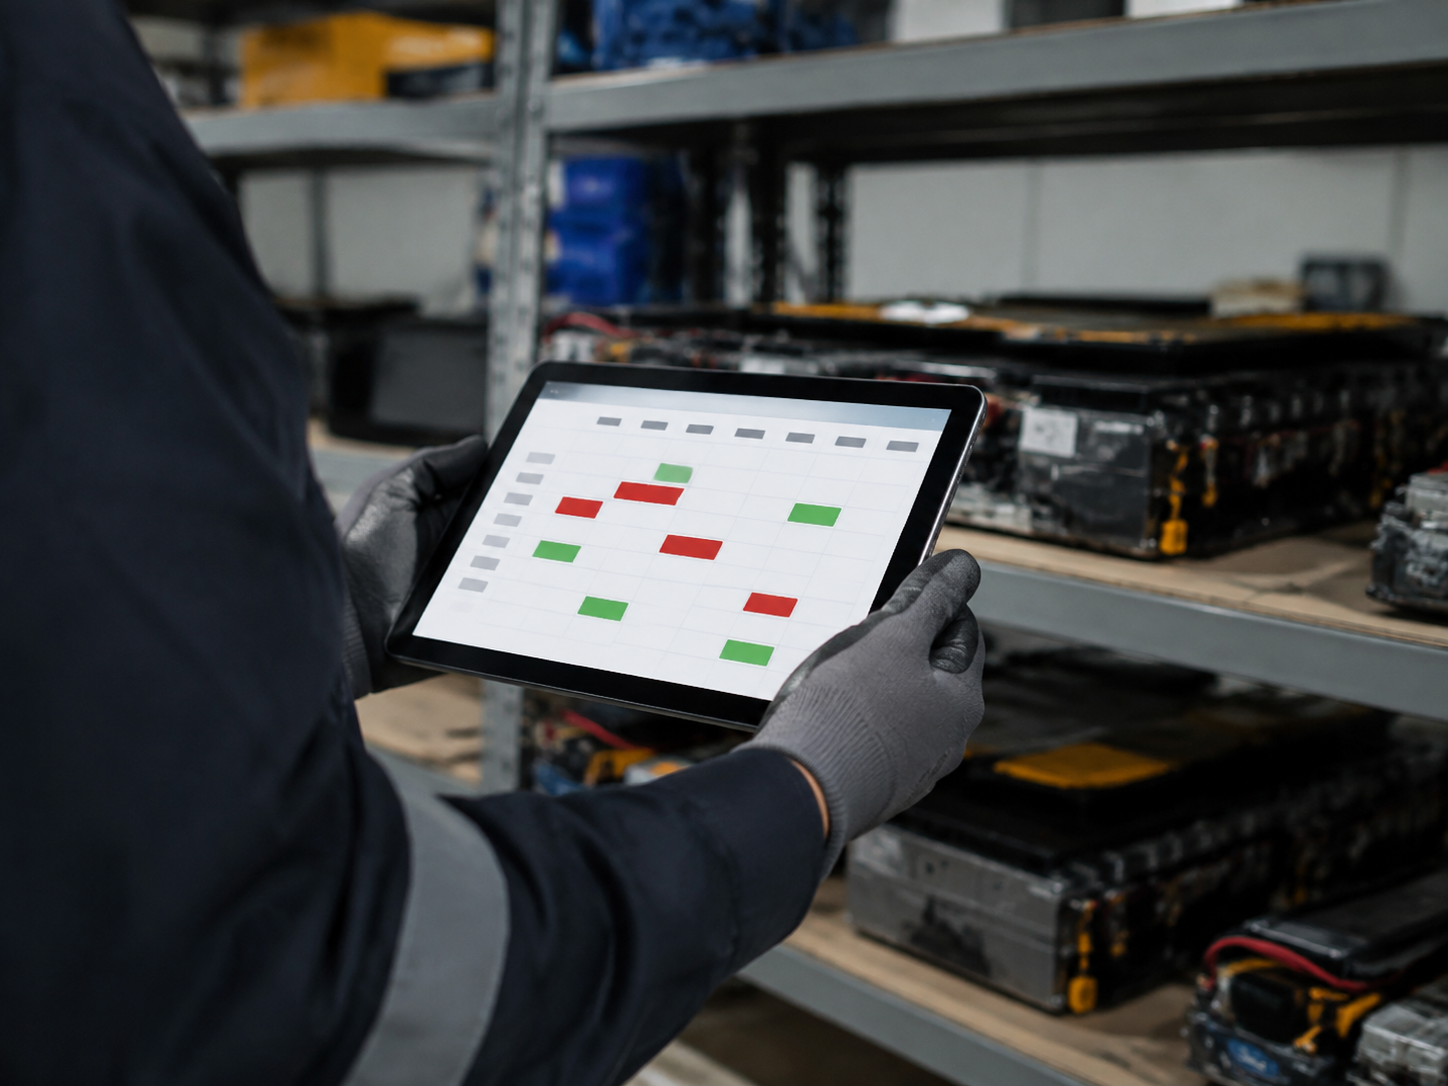
\includegraphics[width=\linewidth]{figures/ov_p3c}
\caption{Decision-grade UQ}\label{fig:ov_attr_uq}
\end{subfigure}\hfill
\begin{subfigure}[b]{0.235\textwidth}
\centering
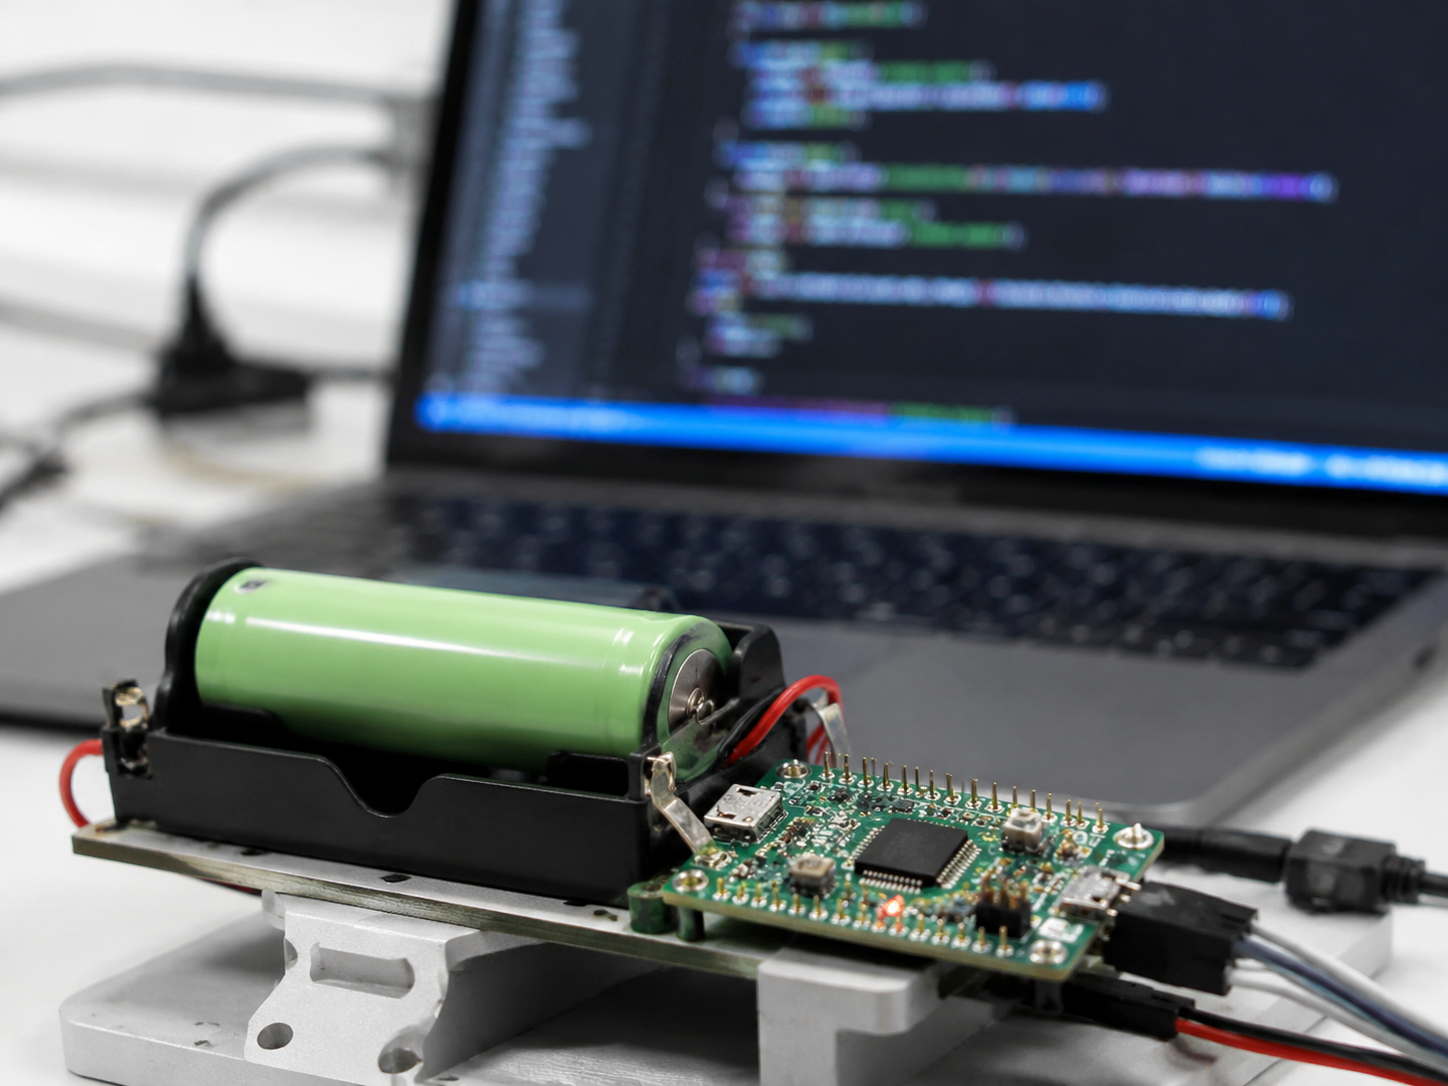
\includegraphics[width=\linewidth]{figures/ov_p3d}
\caption{Edge deployment}\label{fig:ov_attr_edge}
\end{subfigure}
\caption{System overview. Top row: six deployment-context scenes
whose monitoring needs stress a specific capability (shared e-bike
swap, second-life grading, portable medical, EV fleets, robot
fleets, power tools). Middle row: the pipeline---train once per
(dataset, starting point, seed) with min--max input and per-window
z-score targets, the multi-scale GDN-2 model, and per-cycle on-device
inference. Bottom row: four connected capabilities: (A) first-tier
trajectory accuracy including regeneration tracking; (B) a
physics-consistent rate head---physics added to the model, validated
on unseen-tail extrapolation and corrupted field data; (C)
conformal-calibrated P2.5/P50/P97.5 intervals (95\% nominal $\to$
93.3\% actual coverage) for risk-aware maintenance scheduling; and
(D) edge deployment on a microcontroller (16\,KB fixed state,
340\,KB INT8, no dynamic allocation, no cloud).}
\label{fig:overview}
\end{figure}

The technical contributions above translate into an operational
value chain in which each application stresses a specific DeltaCycle
capability rather than generic monitoring (Figure~\ref{fig:overview}):
no-connectivity edge deployment (EV fleets, robot fleets, power
tools/consumer packs with on-pack MCU gauges), risk-aware scheduling
with calibrated intervals (portable medical devices, shared e-bike
swap fleets), and regeneration tracking for non-monotonic field
histories (second-life grading). We stress that the experimental
validation in this paper is conducted on public laboratory cycling
data; the figure is an \emph{application outlook}, not a deployment
report.



The remainder of this paper is organized as follows.
Section~\ref{sec:related} reviews related work.
Section~\ref{sec:method} describes the proposed architecture.
Section~\ref{sec:exp} presents datasets, evaluation protocols, and
experimental results, including ablations, comparison with
PatchFormer, and deployment validation.
Section~\ref{sec:conclusion} concludes the paper.
